\chapter{Graph Attention Networks Embedded Knowledge Tracing Model With Transformer}

% **************************** Define Graphics Path **************************
\ifpdf
    \graphicspath{{Chapter3/Figs/Raster/}{Chapter3/Figs/PDF/}{Chapter3/Figs/}}
\else
    \graphicspath{{Chapter3/Figs/Raster/}{Chapter3/Figs/Vector/}{Chapter3/Figs/PDF/}{Chapter3/Figs/}}
\fi

\section{Research Motivation}
%本章节为该推荐系统的一个核心部分,即通过知识追踪的方式获取学生的知识掌握状态。知识追踪是根据学生的以往的答题记录来建模学生的知识掌握情况,从而获取学生的知识状态。知识追踪的模型非常丰富,早期的知识追踪模型贝叶斯知识追踪(BKT),它们的基础假设是学生答题基于一系列知识点,这些知识点之间被认为是相互不相关的,因此它们之间是独立表示,这种做法无法捕捉不同概念之间的关系也无法表征复杂的概念转换。在2015年,Piech等人提出了深度知识追踪模型(DKT),首次将长短期记忆网络(LSTM)应用于知识追踪任务,它无需进行知识点标注,而是包含一个知识的隐含状态,当时取得了超过BKT的基线性能,它标志着基于神经网络模型的知识追踪研究的序幕。但DKT无法输出知识的隐藏状态,可解释性不足。而且DKT用将所有记忆存储于一个隐藏向量中,对于长序列的预测性能不够理想。针对这个问题,记忆增强网络(MANN)被提出来,它允许网络保留多个隐藏状态向量,并分别读写这些向量。在2017年,张等人提出了Dynamic Key-Value Memory Networks(DKVMN),它参考了MANN的设计,针对知识追踪任务进行了优化,优化了MANN对于知识追踪任务的输入输出不同域的问题。DKVMN采用了键值对作为存储器结构,能避免过拟合、参数少,以及通过潜在概念自动发现相似练习,取得了相对BKT和DKT更好的预测性能。同时该模型也具有较好的可解释性,它将问题相关潜在概念存储于键矩阵中,对概念掌握程度存储于值矩阵中,通过对输入练习与键矩阵的相关性对值矩阵进行更新。

%尽管该模型取得了较好的性能,但该模型将知识点建模为相互独立的点,而未考虑知识点之间的关联性。在高中数学知识网络中,知识点与知识点间有网状的关联关系,而习题是基于这些知识点建立的。因此习题与习题之间也存在隐含的间接关联关系,因此设计一种将考虑知识点间关联的模型来表征该模型是一种合理的解决方案。除了考虑习题知识点的掌握程度,对于学生的答题行为也可以作为额外的特征加入该模型,这样可以为模型增加更多的考虑因素,从而增强模型的预测性能。本文提出了一种用图神经网络结合记忆增强网络的知识追踪模型。该模型相对于原始的DKVMN模型,用图神经网络改造了知识点表征矩阵,并将学生的额外答题行为特征作为模型输入。

This section is a core part of this recommendation system to obtain the student's knowledge mastery status using knowledge tracing. Knowledge tracing is used to model students' knowledge mastery based on their previous answer records to obtain their knowledge status. There is a wealth of models for knowledge tracing, early models of knowledge tracing Bayesian Knowledge Tracing (BKT)~\cite{yudelson2013individualized}, which issued the assumption that students' solutions to exercises are based on a set of knowledge points that are considered to be unrelated to each other and are therefore represented independently of each other. This approach fails to capture the relationships between different concepts nor to characterize complex conceptual transformations. In 2015, Piech et al. proposed the deep knowledge tracing model (DKT), which first applied RNN to the knowledge tracing task, which contains an implicit state of knowledge, and achieved a baseline performance over BKT at that time, and it marked the prologue of knowledge tracing research based on neural network models. However, DKT cannot output the hidden state of knowledge and is not sufficiently interpretable.
Moreover, DKT uses to store all memories in a hidden vector, and the prediction performance for long sequences is not satisfactory enough. Memory Augmented Neural Network (MANN)~\cite{santoro2016meta} was proposed to address this problem, which allows the network to keep multiple hidden state vectors and read and write these vectors separately. In 2017, Dynamic Key-Value Memory Networks (DKVMN)~\cite{zhang2017dynamic} referring to the design of MANN for knowledge tracing tasks and optimizes MANN for knowledge tracing tasks with different input and output domains. DKVMN uses key-value pairs as the memory structure, which can avoid over better prediction performance relative to BKT, and DKT is achieved by using key-value pairs as the memory structure, which can avoid overfitting. The model also has better interpretability. It stores the problem-related potential concepts in the key matrix and the mastery proficiency to the concepts in the value matrix and updates the value matrix by correlating the input exercises with the key matrix.

Although the model achieved better performance, the model modeled knowledge points as mutually independent points without considering the correlations. There are web-like correlations between knowledge points in the high school mathematics knowledge network, and the exercises are built based on these knowledge points. Therefore, there are also implicit and indirect correlations between the exercises and the exercises, so it is reasonable to design a model that will consider the correlations between knowledge points to characterize the model. In addition to considering the degree of mastery of the exercises' knowledge points, the students' answering behaviors can also be added to the model as additional features, adding more considerations to the model and thus enhancing the model's predictive performance. This thesis proposes a knowledge tracking model using graph neural networks combined with memory enhancement networks. The model transforms the knowledge point representation matrix with graph neural networks relative to the original DKVMN model and uses additional characteristics of students' answering behaviors as model inputs.


\section{Related Theory}
\subsection{Knowledge Tracing}
%知识追踪为智能化和自适应教育提供了条件,它具有个性化和自动化的特点。知识追踪任务从学生的历史学习记录来追踪学生的知识状态变化,预测未来的学习表现,从而针对性地给予学习辅导。其本质基于学生的过去的学习表现来获取当前的学习状态,从而预测将来的学习表现。其实际做法是,对学生过去的答题记录进行数据分析和过程建模,从而建模当前的学生学习状态数据,让模型跟做学生的每个阶段的学习状态,并基于学习状态数据来预测习题答对的概率。在学科学习中,学科知识由一系列知识点组成,学生的学习状态实际上基于对于各个知识点的掌握情况。而知识追踪一般的形式为给定一个学生的答题序列,该序列由一系列习题构成,习题又与特定的知识点相关联,在知识追踪中的一个基本假设是,学生的答题表现基于对知识点的掌握。而学生的答题表现即可用于反推学生对于各个知识点的掌握情况,即学习状态的掌握情况。

%知识追踪任务的数学表示为一个学生在一个习题序列上的交互式答题记录\(X_t=(x_1,x_2,\ldots,x_t)\),根据该记录通过建模来获取学生的学习状态,并预测学生在下一次练习中的表现$x_{t+1}$。其中$x_t$通常表示为一个有序对$(q_t,a_t)$,有序对表示学生在时间$t$回答了问题$q_t$,$a_t$表示问题的得分情况,也有许多知识追踪任务用答对或答错来表示,此时$a_t$为0或者1,在此情况下,实际上预测的是对于下一个问题回答正确的概率$P(a_{t+1}=1|a_t)$。如图ref{kt1}。

Knowledge tracing provides the conditions for intelligent and adaptive education, which is personalized and automated. Knowledge tracing tracks students' knowledge status from their historical learning records, predicts future learning performance and provides targeted learning coaching. The essence is to obtain the current learning status based on the student's past learning performance to predict the future learning performance. The actual practice is to analyze the data and process modeling of students' past answer records to model the current student learning status data and let the model follow the learning status of students at each stage, and predict the probability of correct answers to the exercises based on the learning status data. In subject learning, subject knowledge consists of a series of knowledge points, and students' learning status is based on their mastery proficiency to each elementary knowledge concept. The general form of knowledge tracing is that given a sequence of student answers, which consists of a series of exercises associated with a specific knowledge point, a fundamental assumption in knowledge tracing is that student performance is based on mastery proficiency to the knowledge concept. The student's performance can be applied to infer the student's mastery proficiency for each knowledge concept, i.e., the mastery proficiency to the learning state.

The mathematical representation of the knowledge tracing task is an interactive answer record \(X_t=(x_1,x_2,\ldots,x_{t-1})\) of a student on an exercise sequence, based on which the student's learning status is obtained by modeling and predicting the student's performance in the next exercise \(x_{t}\). Where \(x_t\) is usually represented as an ordered pair \((q_t,a_t)\), the ordered pair indicates that the student answered the exercise \(q_t\) at time \(t\), and \(a_t\) indicates the score of the exercise, also many knowledge tracing tasks are represented by correct or incorrect answers, when \(a_t\) is 0 or 1. In this case, what is actually predicted is the probability of answering correctly for the next exercise \(P(a_{t}=1|a_{t-1},\ldots,a_1)\). As shown in the figure \figname{\ref{fig:ch3-model-ktdes}}.

\begin{figure}[htbp!]
    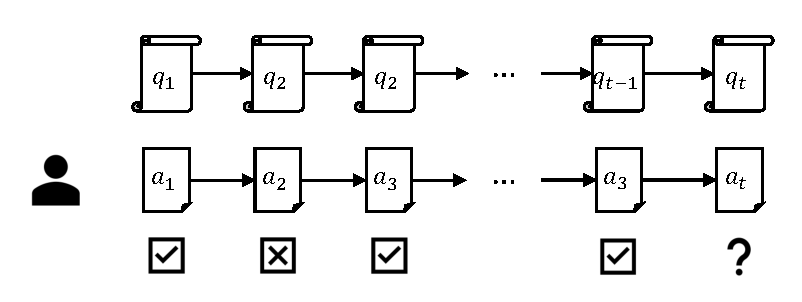
\includegraphics[width=0.9\textwidth]{ch3-kt-model.pdf}
    \caption{The knowledge tracing pattern}\label{fig:ch3-model-ktdes}
\end{figure}

\subsection{Dynamic Key-Value Memory Networks}
%在传统的机器学习模型中,逻辑流控制和外部记忆机制往往缺失。因此,许多当前的机器学习模型无法建立复杂的逻辑流控制和外部记忆模块。传统的模型往往无法高效地利用可训练参数来获得较强记忆能力的模型。目前像LSTM和GRU这些结构,具备一定的记忆能力,但该能力受可训练参数数目影响,记忆增强网络通过更强的表征能力来摆脱可训练参数数目与模型的记忆能力之间的联系。它能够模拟人脑的工作记忆机制,例如阅读理解、推理、运算过程等,也可以捕捉复杂的结构信息和建立长距离信息依赖。MANN将中间信息保留在内存中,形成一个信息缓存结构,并利用该信息进行后续的推理学习。在一个MANN网络中往往分为控制器、存储模块和读写器等三个部分。控制器读取前一阶段的状态和当前的输入来获取下一阶段的输出和控制器输出。存储模块是一个数据结构模型,例如栈、队列或数组,每一个时刻都通过一个输出函数处理读取内容和控制器输出来计算序列输出。

%在知识追踪任务中,由于习题所包含的知识点表征与知识点掌握状态表征所处的空间不同,因此无法将掌握程度和知识点表征用一个存储结构来保存,因此需要对MANN模型进行改造来适配知识追踪任务。DKVMN通过将知识点表征保存在一个矩阵\(M^{(k)}\)中作为Keys,将对应知识点掌握表征保存在另一个矩阵\(M^{(v)}\)中,作为Values。在输入一个习题表示\(q_t\)时,模型将\(q_t\)的嵌入表示向量\(k_t\)与知识点表征模块\(M^{(k)}\)进行相关度计算,得到习题的知识点相关度表示向量\(w_t\)。每个习题都可以表示为一个与知识点的相关度向量,代表了与知识点的相互关系。在DKVMN模型中,有读取过程和写入过程。

%在读取过程中,模型将权重向量\(w_t\)与知识点掌握矩阵\(M^{(v)}\)进行加权和计算,获得用户对于知识点的掌握表征向量\(r_t\)。并将\(r_t\)与当前的习题嵌入向量\(k_t\)进行拼接,经过全联接激活层输\(Tanh(\cdot)\)出\(f_t\),它表示用户对于习题的掌握程度。\(f_t\)会经过一个最终的\(Sigmoid(\cdot)\)激活函数来输出一个习题回答正确的预测概率\(p_t\)。在写入过程中,当前的实际回答表现会对学生的知识掌握状态产生影响,这是一个重新评估的过程。当前的交互记录\(x_t=(q_t,a_t)\)会作为模型的输入。它的嵌入表示\(v_t\)会用于计算知识减少向量\(e_t\)与知识增加向量\(a_t\),减少向量与增加向量会经过与\(w_t\)的加权和作用于\(M^{(v)}\)从而实现对于学生知识状态的更改。训练国歌通过最小化\(p_t\)与习题作答正确性真实标签\(a_t\)的交叉熵损失来进行。整个模型是可微的,因此可以有效利用随机梯度下降来训练。

In traditional machine learning models, logic flow control and external memory mechanisms are often missing. As a result, many current machine learning models cannot build complex logic flow control and external memory modules. Traditional models are often unable to efficiently use trainable parameters to obtain models with strong memory capabilities. Current structures like LSTM and GRU have some memory capability, but that capability is affected by trainable parameters. MANN gets rid of the connection between the number of trainable parameters and the model's memory capability by more robust representational capability. It can simulate the human brain's working memory mechanisms, such as reading comprehension, reasoning, and arithmetic processes, and capture complex structural information and establish long-range information dependencies. MANN keeps intermediate information in memory, forming an information cache structure, and uses that information for subsequent reasoning learning. A MANN network is commonly divided into three parts such as controller, storage module, and reader. The controller reads the previous stage's state and the current input to obtain the next stage's output and the controller output. The storage module is a data structure model, such as a stack, queue, or array, and at each moment, the sequence output is computed by processing the reads and the controller output through an output function.

In the knowledge tracking task, since the knowledge point representations contained in the exercises are in a different space from the knowledge point mastery proficiency state representations, it is not possible to keep the mastery degree and knowledge point representations in one storage structure, so the MANN model needs to be adapted to the knowledge tracking task. In 2017, DKVMN\cite{zhang2017dynamic} was proposed. The DKVMN model is shown in \figname{\ref{fig:ch3-dkvmn-model}}. DKVMN saves the knowledge point representations in a matrix \(M^{(k)}\) as keys by keeping the corresponding knowledge point mastery representations in another matrix \(M^{(k)}\) as Values. The corresponding knowledge point mastery representations are saved in another matrix \(M^{(v)}\) as values. On inputting an exercise representation \(q_t\), the model computes the embedding representation vector \(k_t\) of \(q_t\) with the knowledge point representation module \(M^{(k)}\) to obtain the knowledge point relevance representation vector \(w_t\) of the exercise. Each exercise can be represented as a correlation vector with a knowledge point, representing the interrelationship with the knowledge point. In the DKVMN model, there is a read process and a write process.

\begin{figure}[htbp!]
    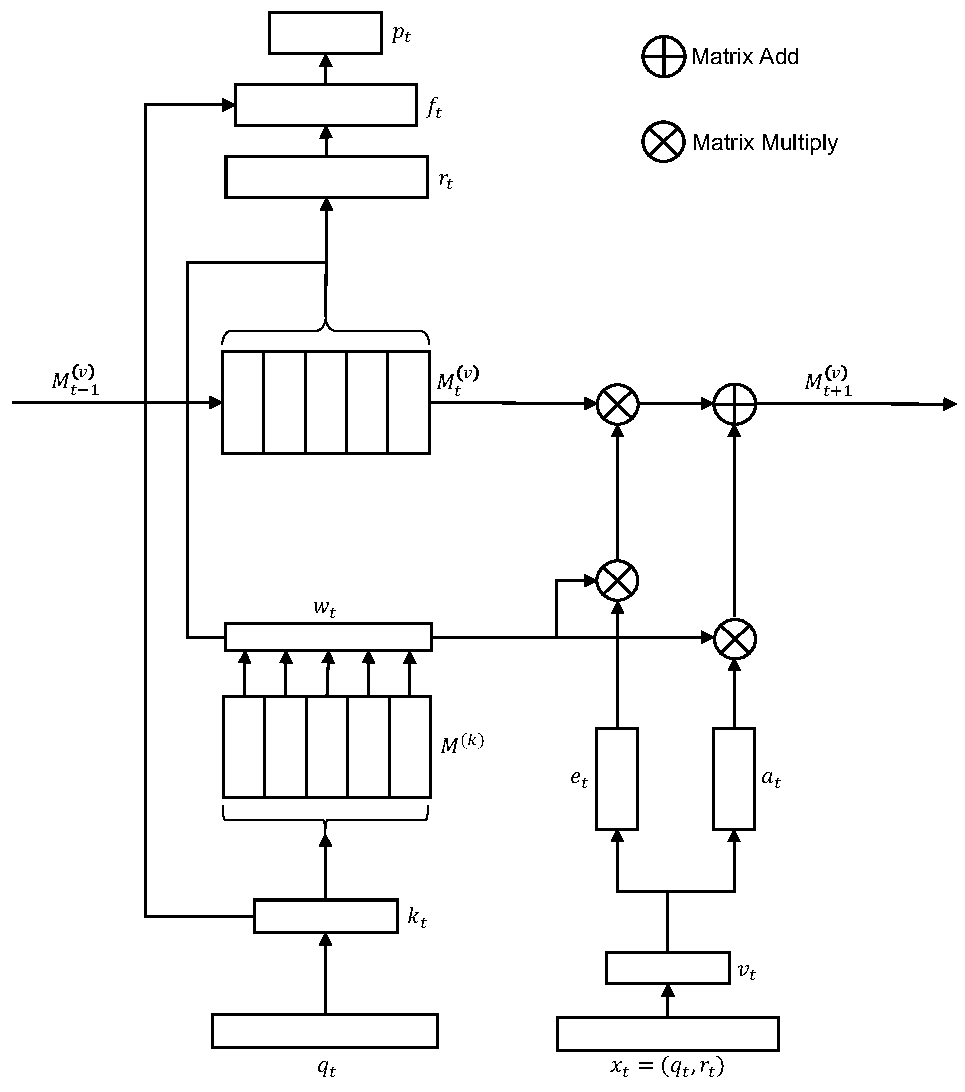
\includegraphics[width=0.9\textwidth]{ch3-dkvmn-model.pdf}
    \caption{The original Dynamic key-value memory network model}\label{fig:ch3-dkvmn-model}
\end{figure}

In the reading process, the model weights and calculates the weight vector \(w_t\) with the knowledge point mastery matrix \(M^{(v)}\) to obtain the user's mastery representation vector \(r_t\) for the knowledge point. And \(r_t\) is spliced with the current exercise embedding vector \(k_t\), and \(f_t\) is derived after the full-linked activation layer loses \(Tanh(\cdot)\), which indicates the user's mastery of the exercise. The \(f_t\) goes through a final \(Sigmoid(\cdot)\) activation function to output a predicted probability of answering the exercise correctly \(p_t\). During the writing process, the current actual response performance will impact the student's knowledge acquisition status, which is a re-evaluation process. The current interaction record \(x_t=(q_t,a_t)\) will be used as the input to the model. Its embedding representation \(v_t\) will be used to compute the knowledge reduction vector \(e_t\) and the knowledge increase vector \(a_t\), and the reduction and increase vectors will be weighted with \(w_t\) and act on \(M^{(v)}\) thus realizing the change for the student's knowledge state. The training process is performed by minimizing the cross-entropy loss of \(p_t\) with the true label \(a_t\) of the correctness of the answers to the exercises. The whole model is microscopic and thus can be trained efficiently using stochastic gradient descent.

\section{Proposed Model}
%DKVMN模型有如下的问题,第一,该模型未考虑学生的特性,每个学生对于潜在知识点的掌握程度会导致不同的结果,即,当两个知识点掌握程度相同的学生可能对于一个习题的作答结果会产生不同的预测度。第二,该模型未考虑知识点的内在联系,该模型将知识点作为存储结构中的一个slot,各个slot之间相互独立。这隔绝了知识点变化引起的相关知识点的变化。在高中数学学科中,有许多相互相关的知识点,因此,需要结合领域特征,加入知识点关联学习网络。本文基于上述两点,对DKVMN模型进行改进。

The DKVMN model has the following problems. First, the model does not take into account the characteristics of students, and each student's mastery of potential knowledge points will lead to different results, i.e., when two students with the same level of mastery of knowledge points may have different prediction degrees for the answer results of an exercise. Second, the model does not consider the intrinsic connection of the knowledge points, which are treated as a slot in the storage structure, and each slot is independent with others. This isolates the changes in related knowledge points caused by changes in knowledge points. In high school mathematics subjects, there are many interrelated knowledge points. Therefore, it is necessary to incorporate the domain characteristics and join the knowledge point associated learning network. In this thesis, the DKVMN model is improved based on the above two points.

\subsection{Algorithm Overview}
%本节的关键点是对学生的知识追踪,本文提出了一种针对DKVMN的改进型知识追踪网络模型,它在原模型的基础上增加了额外的用户答题特征,并通过图网络来改进知识点掌握度表征存储模块,从而为模型增加知识点间关系表征能力。本模型依然具有习题-知识点关联度计算、读取过程、写入过程和知识网络传播过程和预测过程等多个子模块。其模型框架如图。

The key point of this section is the knowledge tracking of students. In this thesis, we propose an improved knowledge tracking network model for DKVMN, which adds additional user answer features to the original model and improves the knowledge point mastery representation storage module by graph networks, thus adding inter-knowledge point relationship representation capability to the model. The model still has several sub-modules such as exercise-knowledge point association degree calculation, reading process, writing process and knowledge network propagation process, and prediction process. Its model framework is shown in \figname{\ref{fig:ch3-gkvmn-model}}.

\begin{figure}[htbp!]
    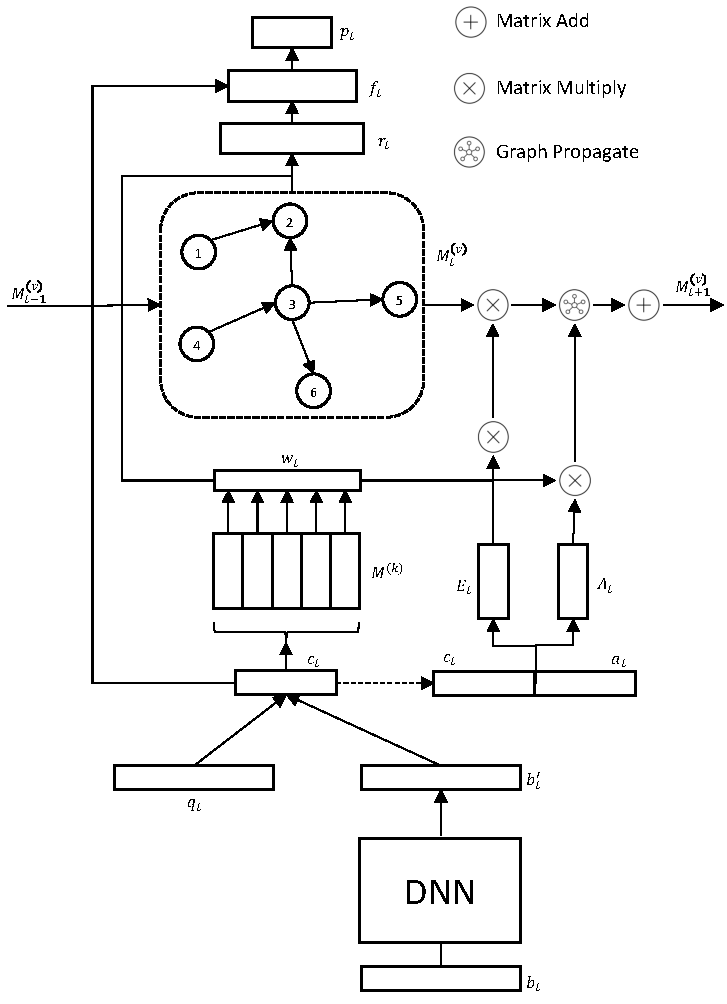
\includegraphics[width=0.9\textwidth]{ch3-gkvmn-model.pdf}
    \caption{Graph key-value memory network architecture}\label{fig:ch3-gkvmn-model}
\end{figure}
\subsection{Student Behavior Capturing}


\subsection{Question Knowledge Correlation Calculation}

\subsection{Transformer Based Knowledge Tracing}

\section{Experiments}
%本节中,通过多个专用的知识追踪数据集来investigate提出的模型性能,与目前已经提出的Baseline模型进行性能对比。本章先对所用到的数据集进行介绍和统计,然后提出用于模型性能对比的度量标准、实验设置和运行参数环境等,最后得出结果并进行分析。
In this section, algorithms, including the performance, are investigated through multiple dedicated knowledge tracing data sets, and the performance of the proposed baseline model is compared. This chapter first introduces and counts the data sets used, then proposes metrics, experimental settings, and operating parameter environments for model performance comparison, and finally draws the results and analyzes them.


\subsection{Datasets}
After investigating the existing knowledge tracing model, the thesis selected the more popular ASSISTment data set and Statics data set related to mathematics, preprocessed the data set, cleaned the data, obtained the training set, and performed the performance with the Baseline model Compared. Dataset statistics are shown in \tblname{\ref{tbl:ch2-tb1}}.

%(1)ASSISTment 2015 是一个用于预测学生考试表现的数据集,它由一系列包含若干知识点标签的问题以及一些学生的答题记录组成。它在2015年于线上教育平台上采集而成。经过数据过滤获得包含19917个学生,约102千个问题,100个知识点标签和约709次交互的数据集。
%(2)ASSISTment 2017 来源于2017年举办的ASSISTments Longitudinal Data Mining Competition。经过数据预处理和数据过滤,数据集包含1709个学生,4117个问题,102个知识点和约943千次交互。
%(3)Statics 2011 数据集来源于统计学课程的答题记录。
\begin{itemize}
    \item ASSISTment 2015 (ASSIST15) is a data set used to predict student test performance. It consists of a series of exercises containing several knowledge point labels and some student answer records. It was collected on an online education platform in 2015. After data filtering, a data set containing 19,917 students, about 102 thousand exercises, 100 knowledge point labels, and about 709 interactions was obtained.
    \item ASSISTment 2017 (ASSIST17) is derived from the ASSISTments Longitudinal Data Mining Competition held in 2017. After data preprocessing and data filtering, the data set contains 1709 students, 4117 exercises, 102 knowledge points, and approximately 943 thousand interactions.
    \item Statics 2011 (STATICS11) dataset is derived from the answer records of statistics courses. It contains 333 students, 1223 exercises, 156 knowledge tags, and about 189 thousand interactions.
\end{itemize}

\begin{table}[htbp!]
    \centering
    \caption{Dataset Statistics}\label{tbl:ch2-tb1}
    \begin{tabular}{ccccc}
        \toprule
        Dataset   & \#Students & \#exercises & \#Knowledge Points & \#Interactions \\
        \midrule
        ASSIST15  & 19,917     & 102,396     & 100                & 709K           \\
        ASSIST17  & 1,709      & 4,117       & 102                & 943K           \\
        STATICS11 & 333        & 1,223       & 156                & 189K           \\
        \bottomrule
    \end{tabular}
\end{table}

\subsection{Settings and Metrics}
%目前知识追踪领域的论文多以(Area Under Curve)AUC作为对比指标,AUC是一个基于ROC曲线常用的二分类评测手段,具有较好的性能对比能力。在知识追踪任务中,最终预测也是当前时刻的习题的做对与否,本质上为一个二分类问题,因此可以采取这种做法。
At present, most papers in the field of knowledge tracing use Area Under Curve (AUC) as a comparison indicator. AUC is a commonly used two-category evaluation method based on the ROC curve and has good performance comparison capabilities. In the task of knowledge tracing, the final prediction is whether the exercises at the current moment are done correctly or not, which is essentially a binary classification problem so that this approach can be adopted.

%对于每个数据集采用70%作为训练集,剩余30%作为测试集。实验运行环境为Ubuntu20.04,TensorFlow 2.23,Python 3.8.6,实验机器为一块Tesla V100计算卡。
For each dataset, 70\% is used as the training set, and the remaining 30\% is taken as the test set. The experimental running environment is Ubuntu20.04, TensorFlow 2.23, Python 3.8.6, and the experimental machine is a Tesla V100 computing card.

\subsection{Baselines}
%1.BKT是一个知识追踪的经典模型,它基于隐马尔可夫模型(HMM),将学习者的知识状态建模为一组对应知识点掌握情况的二元变量。
%2.DKT是第一个基于深度学习的知识追踪模型,它应用将学生的做题记录输入到LSTM中,可以捕获学生做题序列上近期做题记录的影响,将学生的做题顺序考虑进模型,DKT也初步考虑了知识点间的内在相关性。
%3.GKT应用图神经网络到知识追踪任务上,利用图的特性,将知识点间的图状关联表征出来,从而更好地学习知识内在依赖关系,该模型能够学习出学生的隐藏知识状态,也具有较好的可解释性。
In this experiment, baseline performance comparisons are made by comparing some classic models with new knowledge tracing models proposed recently. The following models participate in performance comparison.
\begin{itemize}
    \item BKT~\cite{yudelson2013individualized}: BKT is a probabilistic model that predicts the probability of correctness of answers according to the basic assumption that knowledge points are independent.
    \item DKT~\cite{piech2015deep}: DKT applies the input of students' doing records into LSTM and can capture the influence of recent doing records on students' doing sequences, taking students' doing sequences into account into the model; DKT also initially considers the intrinsic correlation between knowledge points.
    \item Dynamic Key-Value Memory Networks (DKVMN)~\cite{zhang2017dynamic}: DKVMN uses key-value pairs as the memory structure, which can avoid over better prediction performance relative to BKT, and DKT is achieved by using key-value pairs as the memory structure.
    \item Graph-Based Knowledge Tracing (GKT)~\cite{nakagawa2019graph}: GKT applies graphical neural networks to knowledge tracing tasks, using the properties of graphs to characterize the graph-like associations between knowledge points for better learning of intrinsic knowledge dependencies, and the model is able to learn students' hidden knowledge states and also has better interpretability.
\end{itemize}

\subsection{Result and Analysis}
%实验结果见表,相比于其他模型,提出的模型的性能取得了最优的指标。在所有数据集上,DKT、DKVMN和GKT的标签明显优于BKT模型。在ASSIST15数据集上,提出的模型的AUC值较其他模型高出0.5\%,而GKT的性能优于DKVMN和DKT,这是由于该数据集中的知识点隐藏关联较高,因此能够更好表征知识点内在关联的模型就会明显产生更好的结果。在ASSIST17数据集上,提出的模型略优于对比的模型,而DKT、DKVMN和GKT的性能表现差异较小,这是因为知识点间的关联较小,因此考虑知识点间关联带来的性能提升较小。在STATICS11数据集上,DKVMN的性能表现超越了GKT,其原因在于对知识进行关系建模产生了过拟合现象,因此对性能表现产生了负面影响,结果显示出提出的模型抗过拟合性能较好。

The experiment's result is shown in \tblname{\ref{tbl:ch3-tb2}}, and the proposed model achieves better performance metrics than other baseline models. The labels of DKT, DKVMN, and GKT are significantly better than the BKT model on all datasets. On the ASSIST15 dataset, the AUC value of the proposed model is 0.5\% higher than the other models. At the same time, GKT outperforms DKVMN and DKT due to the high hidden association of knowledge points in this dataset, so the model that can better characterize the intrinsic association of knowledge points significantly produces better results. On the ASSIST17 dataset, the proposed model slightly outperforms the compared models. Besides, the performance difference between DKT, DKVMN, and GKT is minor due to the weak association between knowledge points, and thus the performance improvement from considering the association between knowledge points is more diminutive. On the STATICS11 dataset, the performance of DKVMN outperforms GKT due to the overfitting phenomenon arising from modeling the relationship to knowledge, thus negatively affecting the performance, and the results show that the proposed model has better performance against overfitting.

\begin{table}[htbp!]
    \centering
    \caption{AUC results (\%) over three datasets}\label{tbl:ch3-tb2}
    \begin{tabular}{cccc}
        \toprule
        Model    & ASSIST15                    & ASSIST17                   & STATICS11                  \\
        \midrule
        BKT      & \(62.01\pm 0.03 \)          & \(65.30\pm 0.01\)          & \(64.21\pm 0.01\)          \\
        DKT      & \(70.83\pm 0.03 \)          & \(72.66\pm 0.01\)          & \(72.46\pm 0.06\)          \\
        DKVMN    & \(71.06\pm 0.03 \)          & \(72.78\pm 0.02\)          & \(72.67\pm 0.03\)          \\
        GKT      & \(72.12\pm 0.02 \)          & \(72.85\pm 0.01\)          & \(72.57\pm 0.01\)          \\
        \midrule
        Proposed & \(\mathbf{72.62\pm 0.02} \) & \(\mathbf{72.89\pm 0.02}\) & \(\mathbf{72.73\pm 0.02}\) \\
        \bottomrule
    \end{tabular}
\end{table}
\section{Summary}
%
In this section, a knowledge tracing model based on graph self-attentive network hungry embedding with Transformer is proposed, which learns the relationship between exercises and knowledge points through GAT, which can effectively characterize the complex dependencies between knowledge points and can discover the hidden knowledge points in the exercises. In the encoding part, the embedding vectors learned by GAT are encoded by a Transformer model for knowledge state, and a knowledge state sequence is an output, which can be used in the subsequent exercise recommendation process. Also, the knowledge state sequence and the exercises are used as the subsequent decoder's input to output a simulation of the correct or incorrect answers to the exercises.

The innovation points of this section are as follows.
\begin{enumerate}
    \item Based on the graph self-attentive network, a relational graph network with separation of exercises and knowledge points are designed, and the knowledge state embeddings learned in this way can better characterize the intrinsic dependencies of knowledge points.
    \item Through the encoder based on Transformer block, the intrinsic knowledge state vector of students is output, and this state vector can be used for subsequent learning resource recommendation.
    \item With the Transformer block, bidirectional sequence information can be learned better to model students' knowledge states' change.
\end{enumerate}

The model is experimentally verified to achieve good prediction performance for both datasets with closely linked knowledge points and those with sparse knowledge point relationships, and overfitting can also be prevented by proper tuning of parameters.